\section{Growth of Satellite Constellations} \label{sec:satellite-constellations}

Recent years saw a rapid development of satellite technology, especially due to
the growing demand of global connectivity and communication. Therefore,
companies constructed their own satellite constellations leading to a total
number of more than 29'000 objects (according to N2YO in September 2024) in
space at the time of writing.

\begin{figure}[ht]
	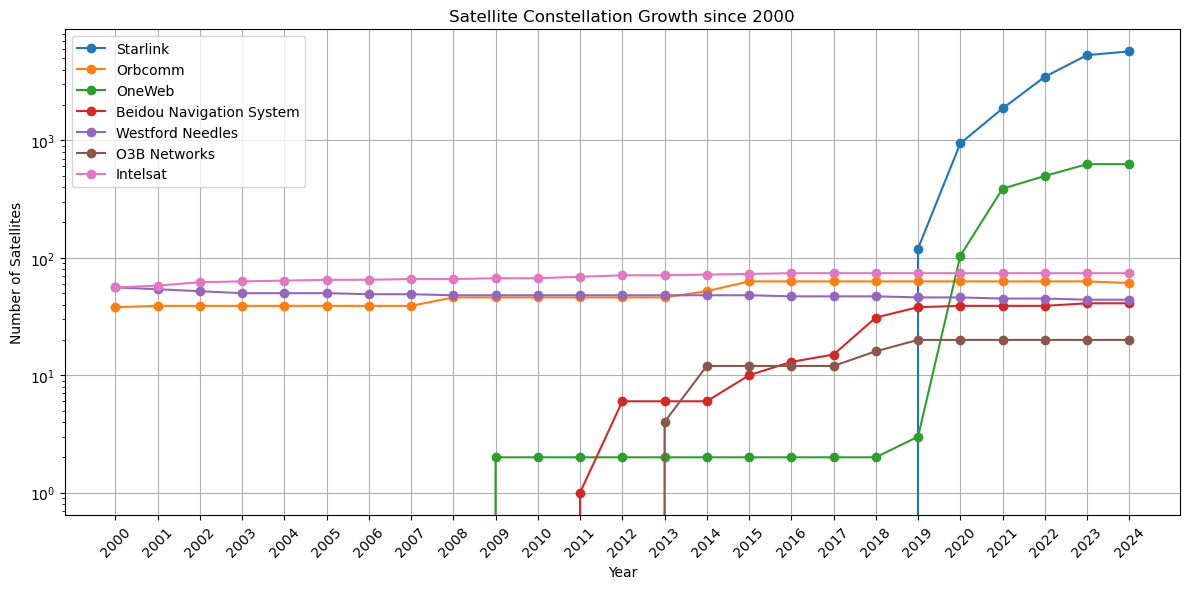
\includegraphics[width=\textwidth]{./chapters/2-background/satellites/img/sattelite-dev.png}
	\caption{Growth of number of satellites in different satellite constellation from 2000 to 2024 (note the logarithmic scale).}
	\label{fig:growth-satellite-constellations}
\end{figure}

\begin{table}
	\caption{Growth of various satellite constellations from 2017 to 2024}
	\label{fig:satellite-constellations-short}
	\begin{tabular}{lrrrrrrrr}
		\toprule
		                          & 2017 & 2018 & 2019 & 2020 & 2021 & 2022 & 2023 & 2024 \\
		Classification            &      &      &      &      &      &      &      &      \\
		\midrule
		\textbf{Starlink}         & 0    & 0    & 120  & 943  & 1871 & 3481 & 5326 & 6396 \\
		\textbf{Orbcomm}          & 63   & 63   & 63   & 63   & 63   & 63   & 63   & 61   \\
		\textbf{OneWeb}           & 2    & 2    & 3    & 104  & 388  & 498  & 628  & 628  \\
		\textbf{Beidou}           & 15   & 31   & 38   & 39   & 39   & 39   & 41   & 41   \\
		\textbf{Westford Needles} & 47   & 47   & 46   & 46   & 45   & 45   & 44   & 44   \\
		\textbf{O3B Networks}     & 12   & 16   & 20   & 20   & 20   & 20   & 20   & 20   \\
		\textbf{Intelsat}         & 74   & 74   & 74   & 74   & 74   & 74   & 74   & 74   \\
		\bottomrule
	\end{tabular}
\end{table}


Figure~\ref{fig:growth-satellite-constellations} shows various satellite
constellations with the number of satellites it consisted of per year.
Table~\ref{fig:satellite-constellations-short} show the corresponding numbers,
starting in 2017. One can see that Starlink is by far the numerically largest
constellation. At the time of writing, it has 6'396 satellites. The Starlink
constellation grew from 2022 to 2023 by nearly 2000 satellites. OneWeb,
Starlink's closest competitor, has a total of 628 satellites with no change
between 2023 and 2024.

Other satellite communication constellations like Orbcomm or Intelsat did not
grow at all, or even lost satellites. Only Starlink and OneWeb see significant
growth in recent years. However, this is also due to the requirement of LEO
constellations (i.e., Starlink and OneWeb) of having largely more satellites,
compared to GEO constellations (e.g., Intelsat and O3B~Networks).
